\documentclass[journal,12pt,twocolumn]{IEEEtran}
\usepackage{setspace}
\usepackage{gensymb}
\singlespacing
\usepackage[cmex10]{amsmath}
\usepackage{amsthm}
\usepackage{mathrsfs}
\usepackage{txfonts}
\usepackage{stfloats}
\usepackage{bm}
\usepackage{cite}
\usepackage{cases}
\usepackage{subfig}
\usepackage{longtable}
\usepackage{multirow}
\usepackage{enumitem}
\usepackage{mathtools}
\usepackage{tikz}
\usepackage{circuitikz}
\usepackage{verbatim}
\usepackage[breaklinks=true]{hyperref}
\usepackage{tkz-euclide} % loads  TikZ and tkz-base
\usepackage{pstricks-add, pst-xkey, fp}
\usepackage{dsptricks, dspblocks, dspfunctions}
\usepackage{listings}
\usepackage{color}    
\usepackage{array}    
\usepackage{longtable}
\usepackage[newfloat]{minted}
\usepackage{calc}     
\usepackage{multirow} 
\usepackage{hhline}   
\usepackage{ifthen}   
\usepackage{lscape}     
\usepackage{chngcntr}
\DeclareMathOperator*{\Res}{Res}
\renewcommand\thesection{\arabic{section}}
\renewcommand\thesubsection{\thesection.\arabic{subsection}}
\renewcommand\thesubsubsection{\thesubsection.\arabic{subsubsection}}
\newenvironment{code}{\captionsetup{type=listing}}{}
\SetupFloatingEnvironment{listing}{name=Source Code}
\renewcommand\thesectiondis{\arabic{section}}
\renewcommand\thesubsectiondis{\thesectiondis.\arabic{subsection}}
\renewcommand\thesubsubsectiondis{\thesubsectiondis.\arabic{subsubsection}}
\renewcommand\thetable{\arabic{table}}
% correct bad hyphenation here
\hyphenation{op-tical net-works semi-conduc-tor}
\def\inputGnumericTable{}                                 %%

\lstset{
%language=C,
frame=single, 
breaklines=true,
columns=fullflexible,
literate=
{-}{$\rightarrow{}$}{1},
}
%\lstset{
%language=tex,
%frame=single, 
%breaklines=true
%}

\DeclareMathOperator*{\argmax}{arg\,max}
\DeclareMathOperator*{\argmin}{arg\,min}
\begin{document}
\newtheorem{theorem}{Theorem}[section]
\newtheorem{problem}{Problem}
\newtheorem{proposition}{Proposition}[section]
\newtheorem{lemma}{Lemma}[section]
\newtheorem{corollary}[theorem]{Corollary}
\newtheorem{example}{Example}[section]
\newtheorem{definition}[problem]{Definition}
\newcommand{\BEQA}{\begin{eqnarray}}
\newcommand{\EEQA}{\end{eqnarray}}
\newcommand{\define}{\stackrel{\triangle}{=}}
\bibliographystyle{IEEEtran}
\providecommand{\mbf}{\mathbf}
\providecommand{\pr}[1]{\ensuremath{\Pr\left(#1\right)}}
\providecommand{\qfunc}[1]{\ensuremath{Q\left(#1\right)}}
\providecommand{\sbrak}[1]{\ensuremath{{}\left[#1\right]}}
\providecommand{\lsbrak}[1]{\ensuremath{{}\left[#1\right.}}
\providecommand{\rsbrak}[1]{\ensuremath{{}\left.#1\right]}}
\providecommand{\brak}[1]{\ensuremath{\left(#1\right)}}
\providecommand{\lbrak}[1]{\ensuremath{\left(#1\right.}}
\providecommand{\rbrak}[1]{\ensuremath{\left.#1\right)}}
\providecommand{\cbrak}[1]{\ensuremath{\left\{#1\right\}}}
\providecommand{\lcbrak}[1]{\ensuremath{\left\{#1\right.}}
\providecommand{\rcbrak}[1]{\ensuremath{\left.#1\right\}}}
\theoremstyle{remark}
\newtheorem{rem}{Remark}
\newcommand{\sgn}{\mathop{\mathrm{sgn}}}
\providecommand{\abs}[1]{\left\vert#1\right\vert}
\providecommand{\res}[1]{\Res\displaylimits_{#1}} 
\providecommand{\norm}[1]{\left\lVert#1\right\rVert}
\providecommand{\mtx}[1]{\mathbf{#1}}
\providecommand{\mean}[1]{E\left[ #1 \right]}   
\providecommand{\fourier}{\overset{\mathcal{F}}{ \rightleftharpoons}}
\providecommand{\system}[1]{\overset{\mathcal{#1}}{ \longleftrightarrow}}
\newcommand{\solution}{\noindent \textbf{Solution: }}
\newcommand{\cosec}{\,\text{cosec}\,}
\providecommand{\dec}[2]{\ensuremath{\overset{#1}{\underset{#2}{\gtrless}}}}
\newcommand{\myvec}[1]{\ensuremath{\begin{pmatrix}#1\end{pmatrix}}}
\newcommand{\mydet}[1]{\ensuremath{\begin{vmatrix}#1\end{vmatrix}}}
\renewcommand{\vec}[1]{\boldsymbol{\mathbf{#1}}}
\def\putbox#1#2#3{\makebox[0in][l]{\makebox[#1][l]{}\raisebox{\baselineskip}[0in][0in]{\raisebox{#2}[0in][0in]{#3}}}}
     \def\rightbox#1{\makebox[0in][r]{#1}}
     \def\centbox#1{\makebox[0in]{#1}}
     \def\topbox#1{\raisebox{-\baselineskip}[0in][0in]{#1}}
     \def\midbox#1{\raisebox{-0.5\baselineskip}[0in][0in]{#1}}

\vspace{3cm}
\title{EE5900 Programming Assignment }
\author{Gautam Singh\\CS21BTECH11018}
\maketitle
\tableofcontents
\bigskip

\section{Solutions}

\begin{enumerate}
    \item The given filter is
    \begin{equation}
        y\sbrak{n} = ay\sbrak{n-1} - ax\sbrak{n} + x\sbrak{n-1}.
        \label{eq:ap-filter}
    \end{equation}
    \begin{enumerate}
        \item The direct form II implementation is shown in
        \autoref{fig:ap-df2}.
            
            \begin{figure}[!ht]
                \centering
                \begin{dspBlocks}{0.3}{0.3}
    % first row:
    \(x[n]\) &          & \BDadd   &        & \BDsplit &%
             &          & \BDadd   &        & \(y[n]\) \\
    %
    % second row:
             &          &          &          & \BDdelay &%
             &          &          &          &          \\
    % third row:
             &          &          &          & \BDsplit &%
             &          &          &          &          \\
    %
    % connections:
      \BDConnH{1}{1}{3}{}
      \ncline{1,3}{1,5}\naput{\(v[n]\)}
      \BDConnH{1}{5}{8}{\(-a\)}
      \BDConnH{1}{8}{10}{}
      \BDConnV{3}{3}{1}{}
      \BDConnV{1}{5}{2}{}
      \ncline{2,5}{3,5}
      \ncline{3,3}{3,5}\nbput{\(a\)}
      \ncline{3,5}{3,8}
      \BDConnV{3}{8}{1}{}
\end{dspBlocks}

                \caption{First Order Direct Form II Allpass Filter.}
                \label{fig:ap-df2}
            \end{figure}
        
        \item The reduced multiplication implementation is shown in \autoref{fig:ap-red}.

            \begin{figure}[!ht]
                \centering
                \begin{dspBlocks}{0.3}{0.3}
    % first row:
             &          &          & \BDdelay &          &        &       \\
    %
    % second row:
    \(x[n]\) & \BDsplit & \BDadd   &          & \BDadd   & \BDsplit & \(y[n]\) \\
    %
    % third row:
             &          & \BDdelay &          &          &        &       \\
    %
    % connections:
      \BDConnH{1}{6}{4}{}
      \ncline{1,4}{1,3}
      \BDConnV{1}{3}{2}{}
      \ncline{2,1}{2,2}
      \BDConnH{2}{2}{3}{-1}
      \BDConnH{2}{3}{5}{\(a\)}
      \BDConnH{2}{5}{7}{}
      \ncline{2,2}{3,2}
      \ncline{2,6}{1,6}
      \BDConnH{3}{2}{3}{}
      \ncline{3,3}{3,5}
      \BDConnV{3}{5}{2}{}
\end{dspBlocks}

                \caption{Reduced First Order Allpass Filter.}
                \label{fig:ap-red}
            \end{figure}

        \item \autoref{code:q1-c} generates the outputs in C.

        \item \autoref{code:q1-m} plots the magnitude and phase response for
        various levels of quantization. The results for direct form II
        implementation are shown in \autoref{fig:res-df2}. The results for
        reduced multiplication implementation are shown in
        \autoref{fig:res-red}.

            \begin{figure}[!ht]
                \centering
                \includegraphics[width=\columnwidth]{figs/q1_fig1.eps}
                \caption{Direct Form II Filter Response for Various Levels of Quantization.}
                \label{fig:res-df2}
            \end{figure}

            \begin{figure}[!ht]
                \centering
                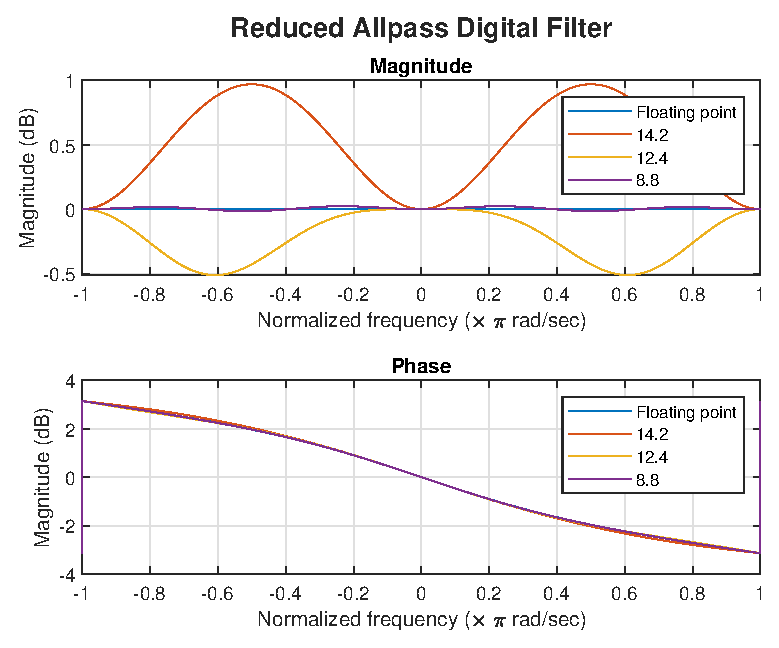
\includegraphics[width=\columnwidth]{figs/q1_fig2.eps}
                \caption{Reduced Form Filter Response for Various Levels of Quantization.}
                \label{fig:res-red}
            \end{figure}
    \end{enumerate}

    \item The given filter is
    \begin{equation}
        y\sbrak{n} = 0.999y\sbrak{n-1} + x\sbrak{n}.
        \label{eq:q2-filter}
    \end{equation}
    Taking the \(Z\)-transform on both sides of \eqref{eq:q2-filter},
    \begin{align}
        Y\brak{z} &= 0.999z^{-1}Y\brak{z} + X\brak{z} \\
        \implies H\brak{z} &= \frac{Y\brak{z}}{X\brak{z}} = \frac{1}{1 - 0.999z^{-1}}.
        \label{eq:H-z-expr}
    \end{align}
    From \eqref{eq:H-z-expr}, we see that
    \begin{equation}
        h\sbrak{n} = \brak{0.999}^nu\sbrak{n}.
        \label{eq:h-n-expr}
    \end{equation}
    Using \eqref{eq:h-n-expr}, we have
    \begin{align}
        \sum_{n=-\infty}^\infty\abs{h\sbrak{n}}^2 &= \sum_{n=0}^\infty \brak{0.999}^{2n} \\
                                                  &= \frac{1}{1 - \brak{0.999}^2} = 500.25
                                                  \label{eq:sum-h2-n}
    \end{align}
    Therefore, the total quantization output power is (\(B=8\) bits)
    \begin{equation}
        P_{e,f} = \frac{2^{-2B}}{12}\frac{1}{1-\abs{a}^2} \text{ W} = 6.36\times 10^{-4}\text{ W}.
    \end{equation}
    \autoref{code:q2-m} simulates the error signal and computes the output
    quantization power over a number of simulations. The results are shown in
    \autoref{fig:qp-sim}.

    \begin{figure}[!ht]
        \centering
        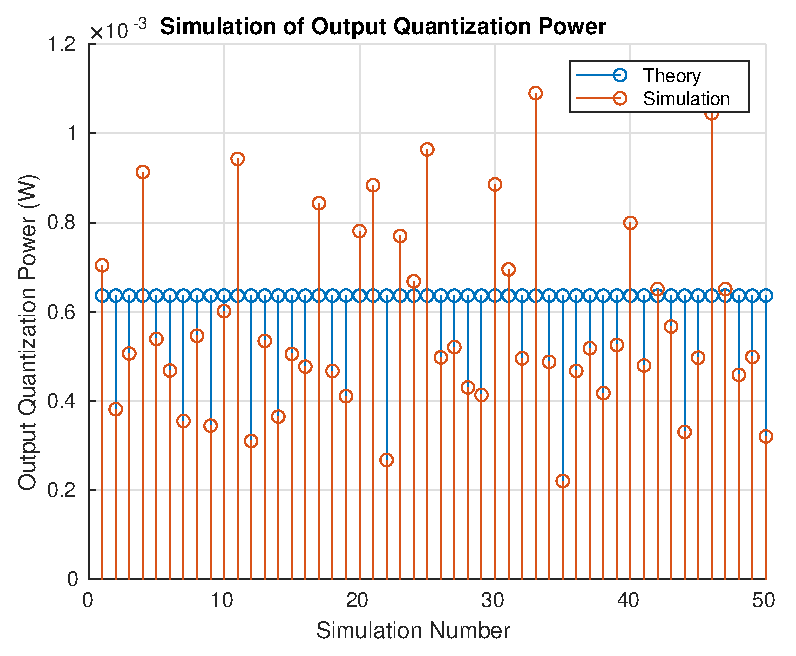
\includegraphics[width=\columnwidth]{figs/q2_fig1.eps}
        \caption{Simulated Quantization Power.}
        \label{fig:qp-sim}
    \end{figure}

    \item The given impulse response is
    \begin{multline}
        h\sbrak{n} = -.375\delta\sbrak{n} + .75\delta\sbrak{n-1} \\
        - .375\delta\sbrak{n-2}.
        \label{eq:q3-impulse}
    \end{multline}
    \begin{enumerate}
        \item Using \eqref{eq:q3-impulse}, the difference equation is
        \begin{multline}
            y\sbrak{n} = -.375x\sbrak{n} + .75x\sbrak{n-1} \\ 
            - .375x\sbrak{n-2}.
            \label{eq:q3-diff-eqn}
        \end{multline}

        Thus, we have
        \begin{align}
            \begin{split}
                y\sbrak{n} &= \abs{-.375x\brak{n}} + \abs{.75x\brak{n-1}} \\
                &+ \abs{-.375x\brak{n-2}}
            \end{split} \\
            \implies y\sbrak{n} &\le \sbrak{.375 + .75 + .375}x_{max} \\
                                &= 1.5x_{max} < 1 \\
        \end{align}
        Hence, \(x_{max} = \frac{1}{1.5} = \frac{2}{3}\).

        \item We have,
        \begin{equation}
            \sum_{n=-\infty}^{\infty}\abs{h\sbrak{n}}^2 = \sum_{n=0}^2\abs{h\sbrak{n}}^2 = 0.84375. \\
        \end{equation}
            Therefore, the output power is (where \(B = 16\) bits)
        \begin{equation}
            P_{e,f} = \frac{2^{-2B}}{12}\sum_{n=-\infty}^{\infty}\abs{h\sbrak{n}}^2 = 1.64\times 10^{-11}\text{ W} 
        \end{equation}
        \autoref{code:q3-m} plots the power spectral density shown in
        \autoref{fig:qp-psd}.
        \begin{figure}[!ht]
            \centering
            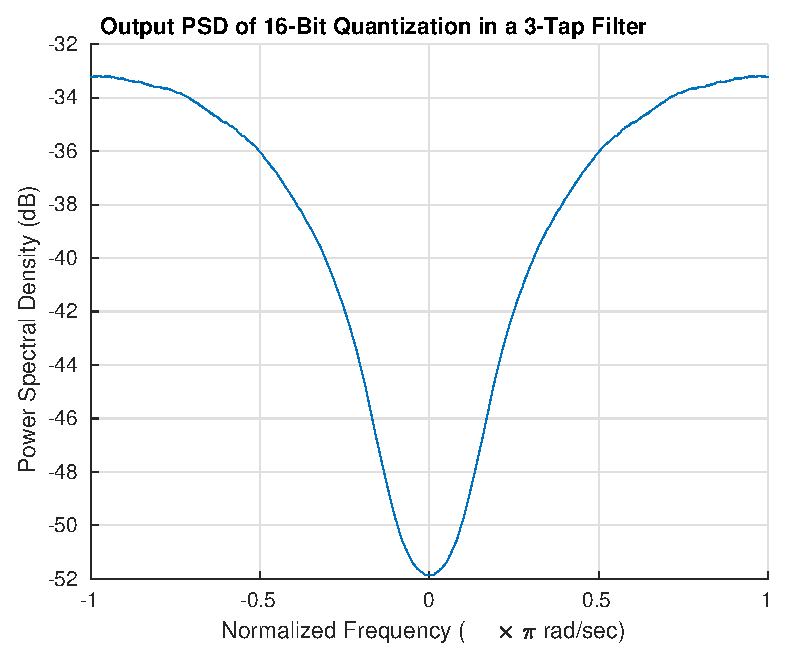
\includegraphics[width=\columnwidth]{figs/q3_fig1.eps}
            \caption{Power Spectral Density of Quantization Noise.}
            \label{fig:qp-psd}
        \end{figure}
    \end{enumerate}
\end{enumerate}

\section{Code}

\begin{code}
    \inputminted[linenos,xleftmargin=1em,breaklines,frame=single]{matlab}{codes/q1.c}
    \captionof{listing}{C Code for Question 1.}
    \label{code:q1-c}
\end{code}

\begin{code}
    \inputminted[linenos,xleftmargin=1em,breaklines,frame=single]{matlab}{codes/q1.m}
    \captionof{listing}{MATLAB Code for Question 1.}
    \label{code:q1-m}
\end{code}

\begin{code}
    \inputminted[linenos,xleftmargin=1em,breaklines,frame=single]{matlab}{codes/q2.m}
    \captionof{listing}{MATLAB Code for Question 2.}
    \label{code:q2-m}
\end{code}

\begin{code}
    \inputminted[linenos,xleftmargin=1em,breaklines,frame=single]{matlab}{codes/q3.m}
    \captionof{listing}{MATLAB Code for Question 3.}
    \label{code:q3-m}
\end{code}
\end{document}
